\chapter{Použití operací nad automaty}
Spojíme znalosti z \ref{chap:Operace} a \ref{chap:Implementace} a podíváme se na použití dříve uvedených operací nad automaty.

Ukázky kódů v této kapitole budou pro lepší čitelnost přebírat syntaxi z reálného kódu. Kapitola se bude soustředit především na sémantickou část a proto budou některé části kódu vynechány. Případně může být vynechána celá implementace, pokud se bude jednat o jednoduchou operaci. Opravdu zanícený čtenář se může vždy podívat do skutečné implementace, jejíž poloha bude uvedena u každého příkladu. Dále v této kapitole už nebudeme používat standardní JavaScript, nýbrž pouze EcmaScript 2015 s Flow a to z důvodů, že by jinak tato kapitola zbytečně nabyla na velikosti. 
\section{Sjednocení (Union)}
Návod jak provést tuto operaci je předveden v předmětu IFJ [TODO reference] a proto se podíváme pouze na její implementaci.
\subsection{Implementace}
V této operaci si ukážeme, nejen jak provést sjednocení, ale jak ho provést nad několika typy automatů. Proto, ikdyž se jedná o relativně jednoduchou operaci, ukážeme si zde její kód.

\begin{lstlisting}[language=JavaScript,label={example:union}, caption={Ukázka implementace operace Union (\textit{src/operations/union.js})}]
{
//@flow
/*Import ptřebných věcí*/

/**
* Sjednocení dvou Automatů
* @param {Automata} left
* @param  {Automata} right
* @return Automata
*/
export default function union(left: (Automata | PA | FA), right: (Automata | PA | FA)) {
	//Převedeme si automat na jeho serializovatelnou reprezentaci
	let plainLeft: T_AnyPlainAutomata = toPlainLeft(left),
			plainRight: T_AnyPlainAutomata = toPlainRight(right);

	// suffix pro nové stavy
	let suffix = State.randomName();


	//sestrojíme automat
	let plainUnion:T_AnyPlainAutomata = {
			states: [{name: 's' + suffix}, /*původní stavy obou automatů*/],
			alphabet: [./*sjednocení abeced*/],
			finalStates: [/*sjednocení koncových stavů*/],
			initialState: {name: 's' + suffix}
	};

	// wrapper pro předávání parametrů
	let paFun = /*funkce pro zásobníkový automat*/;
	// wrapper pro předávání parametrů
	let faFun = /*funkce pro konečný automat*/;

	// Nastavíme jaká funkce se má volat pro kterou kombinaci automatů
	//v tomto případě, pokud je jeden z automatů Zásobníkový, používáme funkci additionalPA
	return overload(
		[
			{parameters: [{value: left, type: FA}, {value: right, type: PA}], func: paFun},
			{parameters: [{value: left, type: PA}, {value: right, type: FA}], func: paFun},
			{parameters: [{value: left, type: PA}, {value: right, type: PA}], func: paFun},
			{parameters: [{value: left, type: FA}, {value: right, type: FA}], func: faFun},
		]
	);
}

\end{lstlisting}
\section{Průnik (Intersection)}
\subsection{Provedení nad automatem}
Průnik dvou Automatů je jednoduchá, avšak dosti zdlouhavá operace. Její aplikaci si předvedmě na příkladu.
Mějme dva automaty :

$M=\{Q_{M}, \Sigma_{M}, R_{M},s_{M}, F_{M}\}$ a $N=\{Q_{N}, \Sigma_{N}, R_{N},s_{N}, F_{N}\} $

Průnik poté provedeme následovně:
\begin{equation}
\label{eqA:Intersection2}
\begin{split}
    Intersection(M,N) = \{ &\\
          &Q = Q_{M} \times Q_{N},\\
    & \tab   \Sigma = \Sigma_{M} \cap \Sigma_{N} \\
    & \tab   R = \{ (q_{M},q_{N})\alpha \longrightarrow (q_{M}\alpha, q_{N}\alpha);\\
    & \tab\tab q_{M} \in Q_{M} \land q_{N} \in Q_{N} \land \alpha \in \Sigma\\
    & \tab\}, \\
    & \tab s = (s_{M}, s_{N}), \\
    & \tab F = F_{M} \times F_{N} \\
    \}&
\end{split}
\end{equation}

\subsection{Implementace}
Implementace zde pouze opisuje postup vytvoření automatu. (Soubor \textit{src/operations/intersectionFA.js})

\section{Doplněk (Complement)}
\subsection{Provedení nad automatem}
Provedení této operace nad automatem vyžaduje aby měl automat takzvaný uklízecí stav (trap state). Uklízecí stav je takový stav, který je nekoncový a jsou do něj odvedeny přechody, které nemohou vést do jiných stavů. Tento stav je dobře popsán v Dobře specifikovaném automatu [TODO reference IFJ]

\subsection{Implementace}
Implementace této operace je ve své podstatě velice jednoduchá, jediné co je potřeba je uvědomit si teorii uvedenou výše, tedy že musíme mít uklízecí stav. Poté pouze uděláme z ukončujících stavů neukončující a naopak.\\
(\textit{src/operations/complementFA.js})
\section{Rozdíl (Difference)}\label{sec:diffImpl}
\subsection{Provedení nad automatem}
Zde pouze sledujeme myšlenku ze sekce \ref{sec:diff} a používáme již existující operace.
\subsection{Implementace}
(\textit{src/operations/differenceFA.js})
\section{Rozdílné sjednocení (Different Union)}
\subsection{Provedení nad automatem}
Hlavní podmínkou provedení této operace je porovnat dva jazyky. Jsme-li schopni rozhodnout o jejich rovnosti, poté je uzavřenost a celková proveditelnost operace ponechána jen proveditelnosti sjednocení. Dva jazyky můžeme považovat za schodné, pokud rozdíl těchto jazyků generuje vždy prázdnou množinu v libovolném pořadí použití. Zde je však vidět, že ne všechny typy jazyků lze porovnávat, jelikož ne všechny typy jazyků jsou uzavřeny nad operací rozdíl. Dva automaty považujeme za shodné, pokud přijímají tentýž jazyk.

\subsection{Implementace}
V implementaci si musíme dávat pozor na porovnávání přijímaných jazyků, avšak pokud se budeme držet teorie a použijeme dříve implementovanou operaci rozdílu. je implementace pouze otázka dvou podmínek.
(\textit{src/operations/differentUnionFA.js})
\section{Operace "Rozdílné" (Operation Different)}
\subsection{Provedení nad automatem}
Provedení je stejné jako nad jazyky, viz \ref{section:OD}, tedy použijeme již existující operace.
\subsection{Implementace}
(\textit{src/operations/operationDifferentFA.js})

\section{Konkatenace (Concatenation)}\label{sec:impConc}
Návod jak provést tuto operaci je předveden v předmětu IFJ [TODO reference] a její implementace je s ní totožná.
\subsection{Implementace}
(\textit{src/operations/concatenationFA.js})
\section{Unikátní Konkatenace (Konkatenace)}
Tato operace lze provést pokud víme jak funguje konkatenace(\ref{sec:impConc}) a rozdíl(\ref{sec:diffImpl}) . Následně můžeme operaci implementovat použitím vzorce \ref{eq:UniqueConcatenation}
\section{Implementace}
(\textit{src/operations/uniqueConcatenationFA.js})
\section{Předpony (Prefixes)}
\subsection{Provedení nad automatem}
Zde je potřeba pouze si uvědomit co je to prefix řetězce. Je prázdý řetězec, první znak, první dva znaky a tak dále, až po poslední znak včetně vice [TODO reference IFJ].  A tedy potřebujeme jen donutit automat aby přijímal všechny řetězce, které mohou vest k řetězci jenž by byl přijat původním automatem. Najdeme si tedy všechny ukončující stavy, uděláme z nich stavy koncové a máme hotovo.

\subsection{Implementace} 
 \begin{lstlisting}[language=JavaScript,caption={Ukázka implementace Předpon (\textit{src/operations/prefixesFA.js})}]
 //@flow
 /*Import potřebných závislostí*/
 
 /**
 * Generuhe automat přijímající prefixy zadaného automatu
 * @param {FA} automata
 * @return {FA}
 */
 export default function prefixes(automata: FA): ?FA {
 	//vytvoříme nový automat ze starého
 	let resAutomata = automata.clone();
 	resAutomata.removeTrapStates(); //odstraníme uklízecí stavy
 
	 //všechny stavy se stávají koncovými
	for(let state of objectValues(resAutomata.states)) {
 		state.setAsFinal();
 	}
 	resAutomata.finalStates = _.clone(resAutomata.states);
 
	 //pro úhlednost přidáme uklízecí stav
	 resAutomata.ensureOneTrapState();
 
	 return resAutomata;
 }
 \end{lstlisting}
\section{(Shuffle)}
\subsection{Provedení nad automatem}
Aplikace se z počátku může zdát složitá. Uvědomíme-li si však, že můžeme používat složení automatů v kartézském součinu pro sledování cesty v kterém automatu se pohybujeme, zjistíme, že stačí provést pouze následující:\\
Mějme dva automaty :

$M=\{Q_{M}, \Sigma_{M}, \delta_{M},s_{M}, F_{M}\}$ a $N=\{Q_{N}, \Sigma_{N}, \delta_{N},s_{N}, F_{N}\} $

Promíchání poté provedeme následovně:
\begin{equation}
\label{eqA:Intersection}
\begin{split}
Shuffle(M,N) = \{ &\\
 & Q = Q_{M} \times Q_{N},\\
 &   \Sigma = \Sigma_{M} \cup \Sigma_{N} \\
    &   \delta = \{ \\
    & \tab (q_{M},q_{N})\alpha \longrightarrow (q_{M}\alpha, q_{N}) \vee (q_{M},q_{N}\alpha);\\
    & \tab q_{M} \in Q_{M} \land q_{N} \in Q_{N} \land \alpha \in \Sigma\\
    & \tab \}, \\
    &  s = (s_{M}, s_{N}), \\
    & F = F_{M} \times F_{N} \\
    & \}
\end{split}
\end{equation}

\subsection{Implementace}
Jak je výše uvedeno v zápisu automatu, promíchání probíhá tak, že se posouváme v dle pravidla automatu $M$, nebo automatu $N$. Viz následující ukázka kódu, kde si ukážeme generování pravidel pro Shuffle.
\begin{lstlisting}[language=JavaScript, caption={Ukázka generování přechodů pro shuffle (\textit{src/operations/shuffleFA.js})}, label=example:shuffle]
/**Anotace*/
function createRules(
	left: FA,
	right: FA,
	newStates: { [key: string]: MergedState }
): Rule[] {
	let newRules = [];
	//pro každý nový stav generujeme pravidla
	for (let newState: MergedState of objectValues(newStates)) {
		//generujeme pravidla z levého automatu
		let leftRules = /*Filtrovaná pravidla levého automatu, pro tento stav*/;
		for (let rule: Rule of leftRules) {
			newRules.push(new Rule({
				from: {state: newState},
				symbol: rule.symbol,
				to: {state: newStates[MergedState.createName(rule.to.state, 	newState.oldRight)]}
			}));
		}

		//generujeme pravidla z pravého automatu
		/*Obdobně jako pro lévé*/
			...
				to: {state: newStates[MergedState.createName(newState.oldLeft, rule.to.state)]}
			...
	}
	return newRules;
}

\end{lstlisting}
\section{Sekvenční Vložení (Sequential Insertion)}
\subsection{Provedení nad automatem}
Vzhledem k faktu, že tato operace je podobná operaci shuffle, můžeme nad ní uvažovat velice podobně. V této operaci je však rozdíl, že musíme vložit řetězec z druhého jazyka nerozdělený. Nejlépe ukážeme na příkladu: 

Mějme dva jazyky $K(M)=\{CD\}$ a $L(N)=\{AA, BB\}$ a automaty kterými jsou definovány.(\ref{imgExample:insertionTeory})
\begin{figure}[H]
\centering
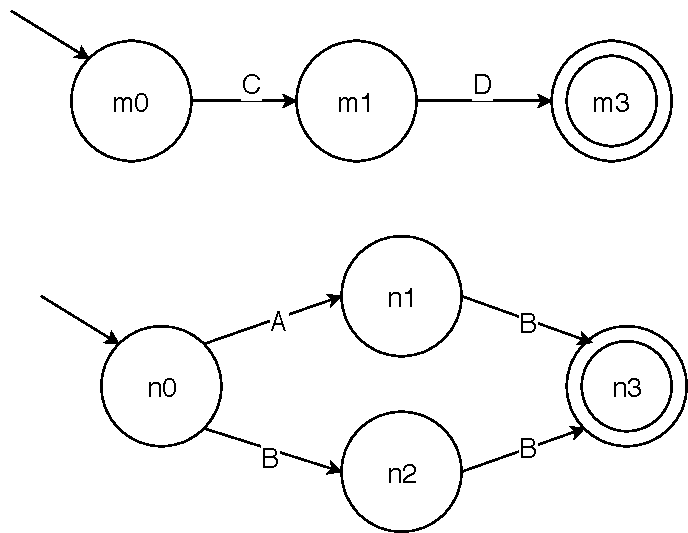
\includegraphics[width=0.7\textwidth]{obrazky-figures/IsertionPriklad.pdf}
\label{imgExample:insertionTeory}
\caption{Příklad automatů pro Sequential Insertion}
\end{figure}

Nyní nad těmito jazyky budeme chtít provést sekvenční vložení $N$ do $M$, tedy \\
$SequentialInsertion(M,N)$. Zde je si potřeba uvědomit, že můžeme provést kartézský součin k tomu abychom sledovali ve kterém jsme právě automatu. Pro jednodušší pochopení si
představme, že automat $M$ je osa $X$ a automat $N$ je osa $Y$. Sekvenční vložení nám pak říká, že musíme řetězec přijímaný automatem $N$ můžeme vložit kamkoliv do řetězce přijímaného automatem $M$. Tedy se můžeme pohybovat přechody po ose $X$
libovolně, ale ve chvíli, kdy se přesuneme po ose $Y$, musíme po této ose dojít až na konec řetězce přijímaného automatem $N$. (viz. \ref{imgExample:insertionTeoryRes})

\begin{figure}[H]
\centering
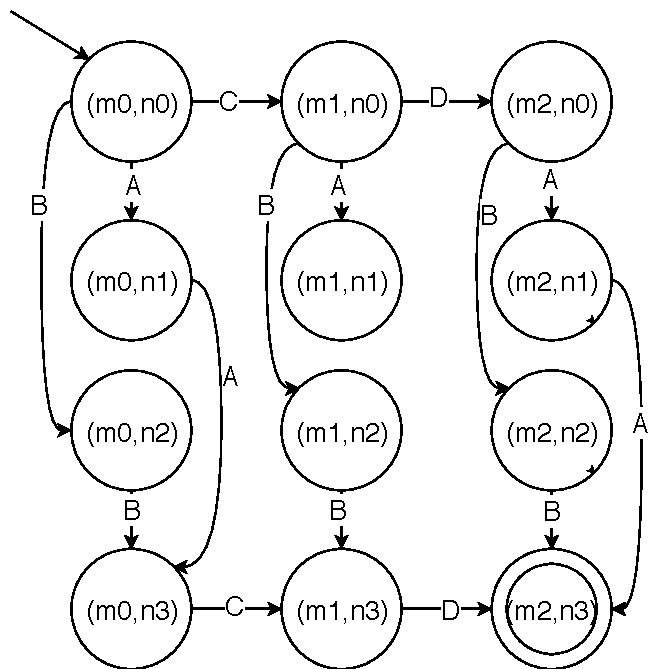
\includegraphics[width=0.7\textwidth]{obrazky-figures/IsertionPrikladResult.pdf}
\label{imgExample:insertionTeoryRes}
\caption{Výsledek po použití operace Sequential Insertion}
\end{figure}



Tento příklad si můžeme zobecnit následujícím způsobem, mějme dva automaty :

$M=\{Q_{M}, \Sigma_{M}, R_{M},s_{M}, F_{M}\}$ a $N=\{Q_{N}, \Sigma_{N}, R_{N},s_{N}, F_{N}\} $

Sekvenční vložení N do M provedeme následovně:
\begin{equation}
\label{eqA:Insertion}
\begin{split}
    Insertion(M,N) = \{ &\\
           &Q = Q_{M} \times Q_{N},\\
    &  \Sigma = \Sigma_{M} \cup \Sigma_{N} \\
    & \delta = \{ (q_{M},q_{N})\alpha \longrightarrow \left\{\begin{matrix}
 (q_{M}\alpha, q_{N})& if & q_{N}=s \vee q_N \in F_{N}\\ 
 (q_{M}, q_{N}\alpha)& else & 
\end{matrix}\right.;\\
    &\tab q_{M} \in Q_{M} \land q_{N} \in Q_{N} \land \alpha \in \Sigma\\
    &\tab\}, \\
    & s = (s_{M}, s_{N}), \\
    & F = F_{M} \times F_{N} \\
    \}&
\end{split}
\end{equation}


\subsection{Implementace}
Pravidla se vytváří dle výše uvedeného automatu, obdobně jako tomu bylo v ukázce \ref{example:shuffle}
(\textit{src/operations/sequentialInsertionFA.js})
% \begin{figure}[h]
% \centering
% \includegraphics[width=0.7\textwidth]{obrazky-figures/intersectionExample.png}
% \label{imgExample:intersection}
% \caption[]
%     {\tabular[t]{@{}l@{}}Ukázka implementace operace Intersection \\ $src/operations/intersectionFA.js$\endtabular}
% \end{figure}

\section{Paralelní vkládání (Paralel Insertion)}
\subsection{Provedení nad automatem}
Provedení paralelního vkládání je velice podobné vkládání sekvenčnímu, nejednodušší bude opět si uvést příklad. Mějme tedy opět dva jazyky $K(M)=\{CD\}$ a $L(N)=\{AA, BB\}$ a automaty kterými jsou definovány, viz výše uvedený příklad pro sekvenční vkládání(\ref{imgExample:insertionTeory});

Rozdíl je zde v tom, že při paralelním vkládání, musíme vždy po zpracování znaku z řetězce jazyka $K(M)$, zpracovat celý řetězec z jazyka $L(N)$. Abychom použili analogii na na osy $X$ a $Y$, tak vždy když se chceme posunout po ose $X$, musíme se posunout po ose $Y$ až do konečného stavu. (viz \ref{imgExample:paralelinsertionResult})
\begin{figure}[H]
\centering
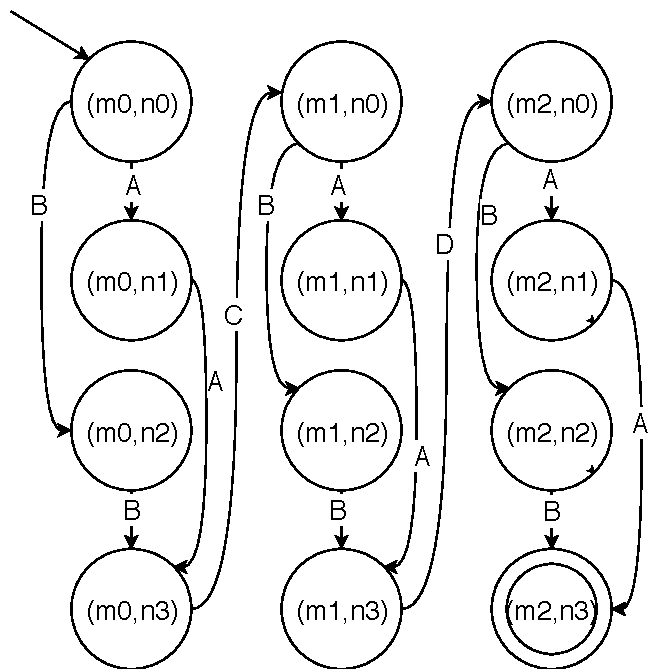
\includegraphics[width=0.7\textwidth]{obrazky-figures/paralelInserionResult.pdf}
\label{imgExample:paralelinsertionResult}
\caption{Automat generovaný operací ParalelInsertion(N,L)}
\end{figure}

Tento příklad si můžeme zobecnit následujícím způsobem, mějme dva automaty :
$M=\{Q_{M}, \Sigma_{M}, \delta_{M},s_{M}, F_{M}\}$ a $N=\{Q_{N}, \Sigma_{N}, \delta_{N},s_{N}, F_{N}\} $

Paralelní vkládání poté můžeme zobecnit následovně:
\begin{equation}
\label{eqA:ParalelInsertion}
\begin{split}
    ParalelInsertion(M,N) = \{ &\\
           &Q = Q_{M} \times Q_{N},\\
    &  \Sigma = \Sigma_{M} \cup \Sigma_{N} \\
    & \delta = \{ (q_{M},q_{N})\alpha \longrightarrow \left\{\begin{matrix}
 (q_{M}\alpha, s_{N})& if & q_N \in F_{N}\\ 
 (q_{M}, q_{N}\alpha)& else & 
\end{matrix}\right.;\\
    &\tab q_{M} \in Q_{M} \land q_{N} \in Q_{N} \land \alpha \in \Sigma\\
    &\tab\}, \\
    & s = (s_{M}, s_{N}), \\
    & F = F_{M} \times F_{N} \\
    \}&
\end{split}
\end{equation}



\subsection{Implementace}
Pravidla se vytváří dle výše uvedeného automatu, obdobně jako tomu bylo v ukázce \ref{example:shuffle}
(\textit{src/operations/parallelInsertionFA.js})
% \begin{figure}[h]
% \centering
% \includegraphics[width=0.7\textwidth]{obrazky-figures/intersectionExample.png}
% \label{imgExample:intersection}
% \caption[]
%     {\tabular[t]{@{}l@{}}Ukázka implementace operace Intersection \\ $src/operations/intersectionFA.js$\endtabular}
% \end{figure}

\section{Protkání (Interlacement)}
V této operaci postupujeme tak, že vytváříme automat přesně tak jak je automat vytvořen v důkazu.
\subsection{Implementace}
Pravidla se vytváří dle výše uvedeného automatu, obdobně jako tomu bylo v ukázce \ref{example:shuffle}
(\textit{src/operations/interlacementFA.js})
\section{Sekvenční mazání (Sequential Deletion)}
[TODO, implementovat, poté popsat]
\section{Zakázání abecedy (Full Alphabet deletion)}
[TODO, implementovat, poté popsat]
[Ale v podstatě se jedná o homomorfismus alpha -> epsilon]
\section{(Pop)}
[TODO, implementovat, poté popsat]
[Ale v podstatě se jedná o homomorfismus alpha -> epsilon]